\section*{Задание 1}
 \subsection*{Постановка задачи}
\textbf{Задание:} Создать базу знаний «Предки», позволяющую \textbf{наиболее эффективным способом}
(за меньшее количество шагов, что обеспечивается меньшим количеством предложений БЗ -
правил), и используя разные варианты (примеры) \textbf{одного вопроса}, определить (указать:
какой вопрос для какого варианта):
\begin{enumerate}
    \item по имени субъекта определить всех его бабушек (предки 2-го колена);
    \item по имени субъекта определить всех его дедушек (предки 2-го колена);
    \item по имени субъекта определить всех его бабушек и дедушек (предки 2-го
	колена);
	\item по имени субъекта определить его бабушку по материнской линии (предки 2-го
	колена);
	\item по имени субъекта определить его бабушку и дедушку по материнской линии
	(предки 2-го колена).
\end{enumerate}

Минимизировать количество правил и количество вариантов вопросов. 
Использовать \textbf{конъюнктивные правила и простой вопрос}.
\textbf{Для одного} из вариантов \textbf{ВОПРОСА} и конкретной БЗ \textbf{составить таблицу},
отражающую конкретный порядок работы системы, с объяснениями:
очередная проблема на каждом шаге и метод ее решения;
каково новое текущее состояние резольвенты, как получено;
какие дальнейшие действия? (Запускается ли алгоритм унификации? Каких термов?
Почему этих?);
вывод по результатам очередного шага и дальнейшие действия.


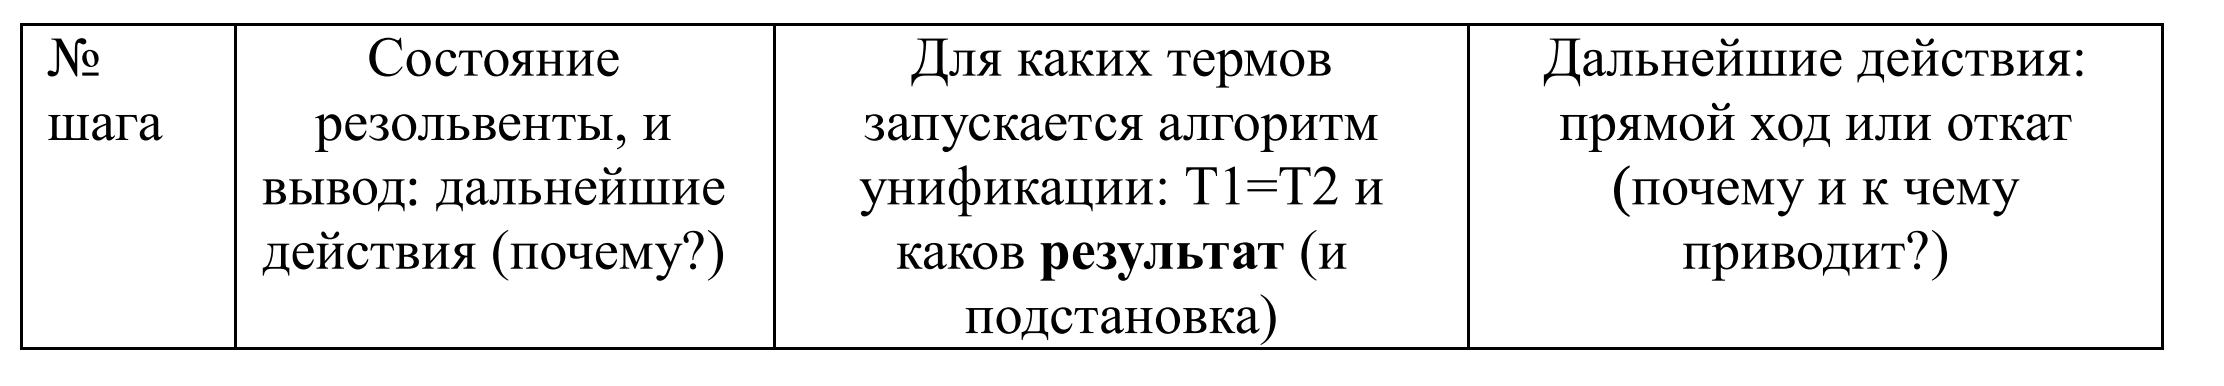
\includegraphics[scale=0.4]{./inc/img/tb_tmpl}


\clearpage
\subsection*{Решение}
\lstinputlisting[
	caption={Задание 1},
	label={lst:t1},
	language=lisp,
	]{../src/main.pro}